% !!! 本文件由 work/tools/build_latex.py 生成，请勿手改 !!!

\begin{center}
\thispagestyle{empty}
\begin{tikzpicture}[remember picture, overlay, inner sep=0pt]
\node at (current page.center)
{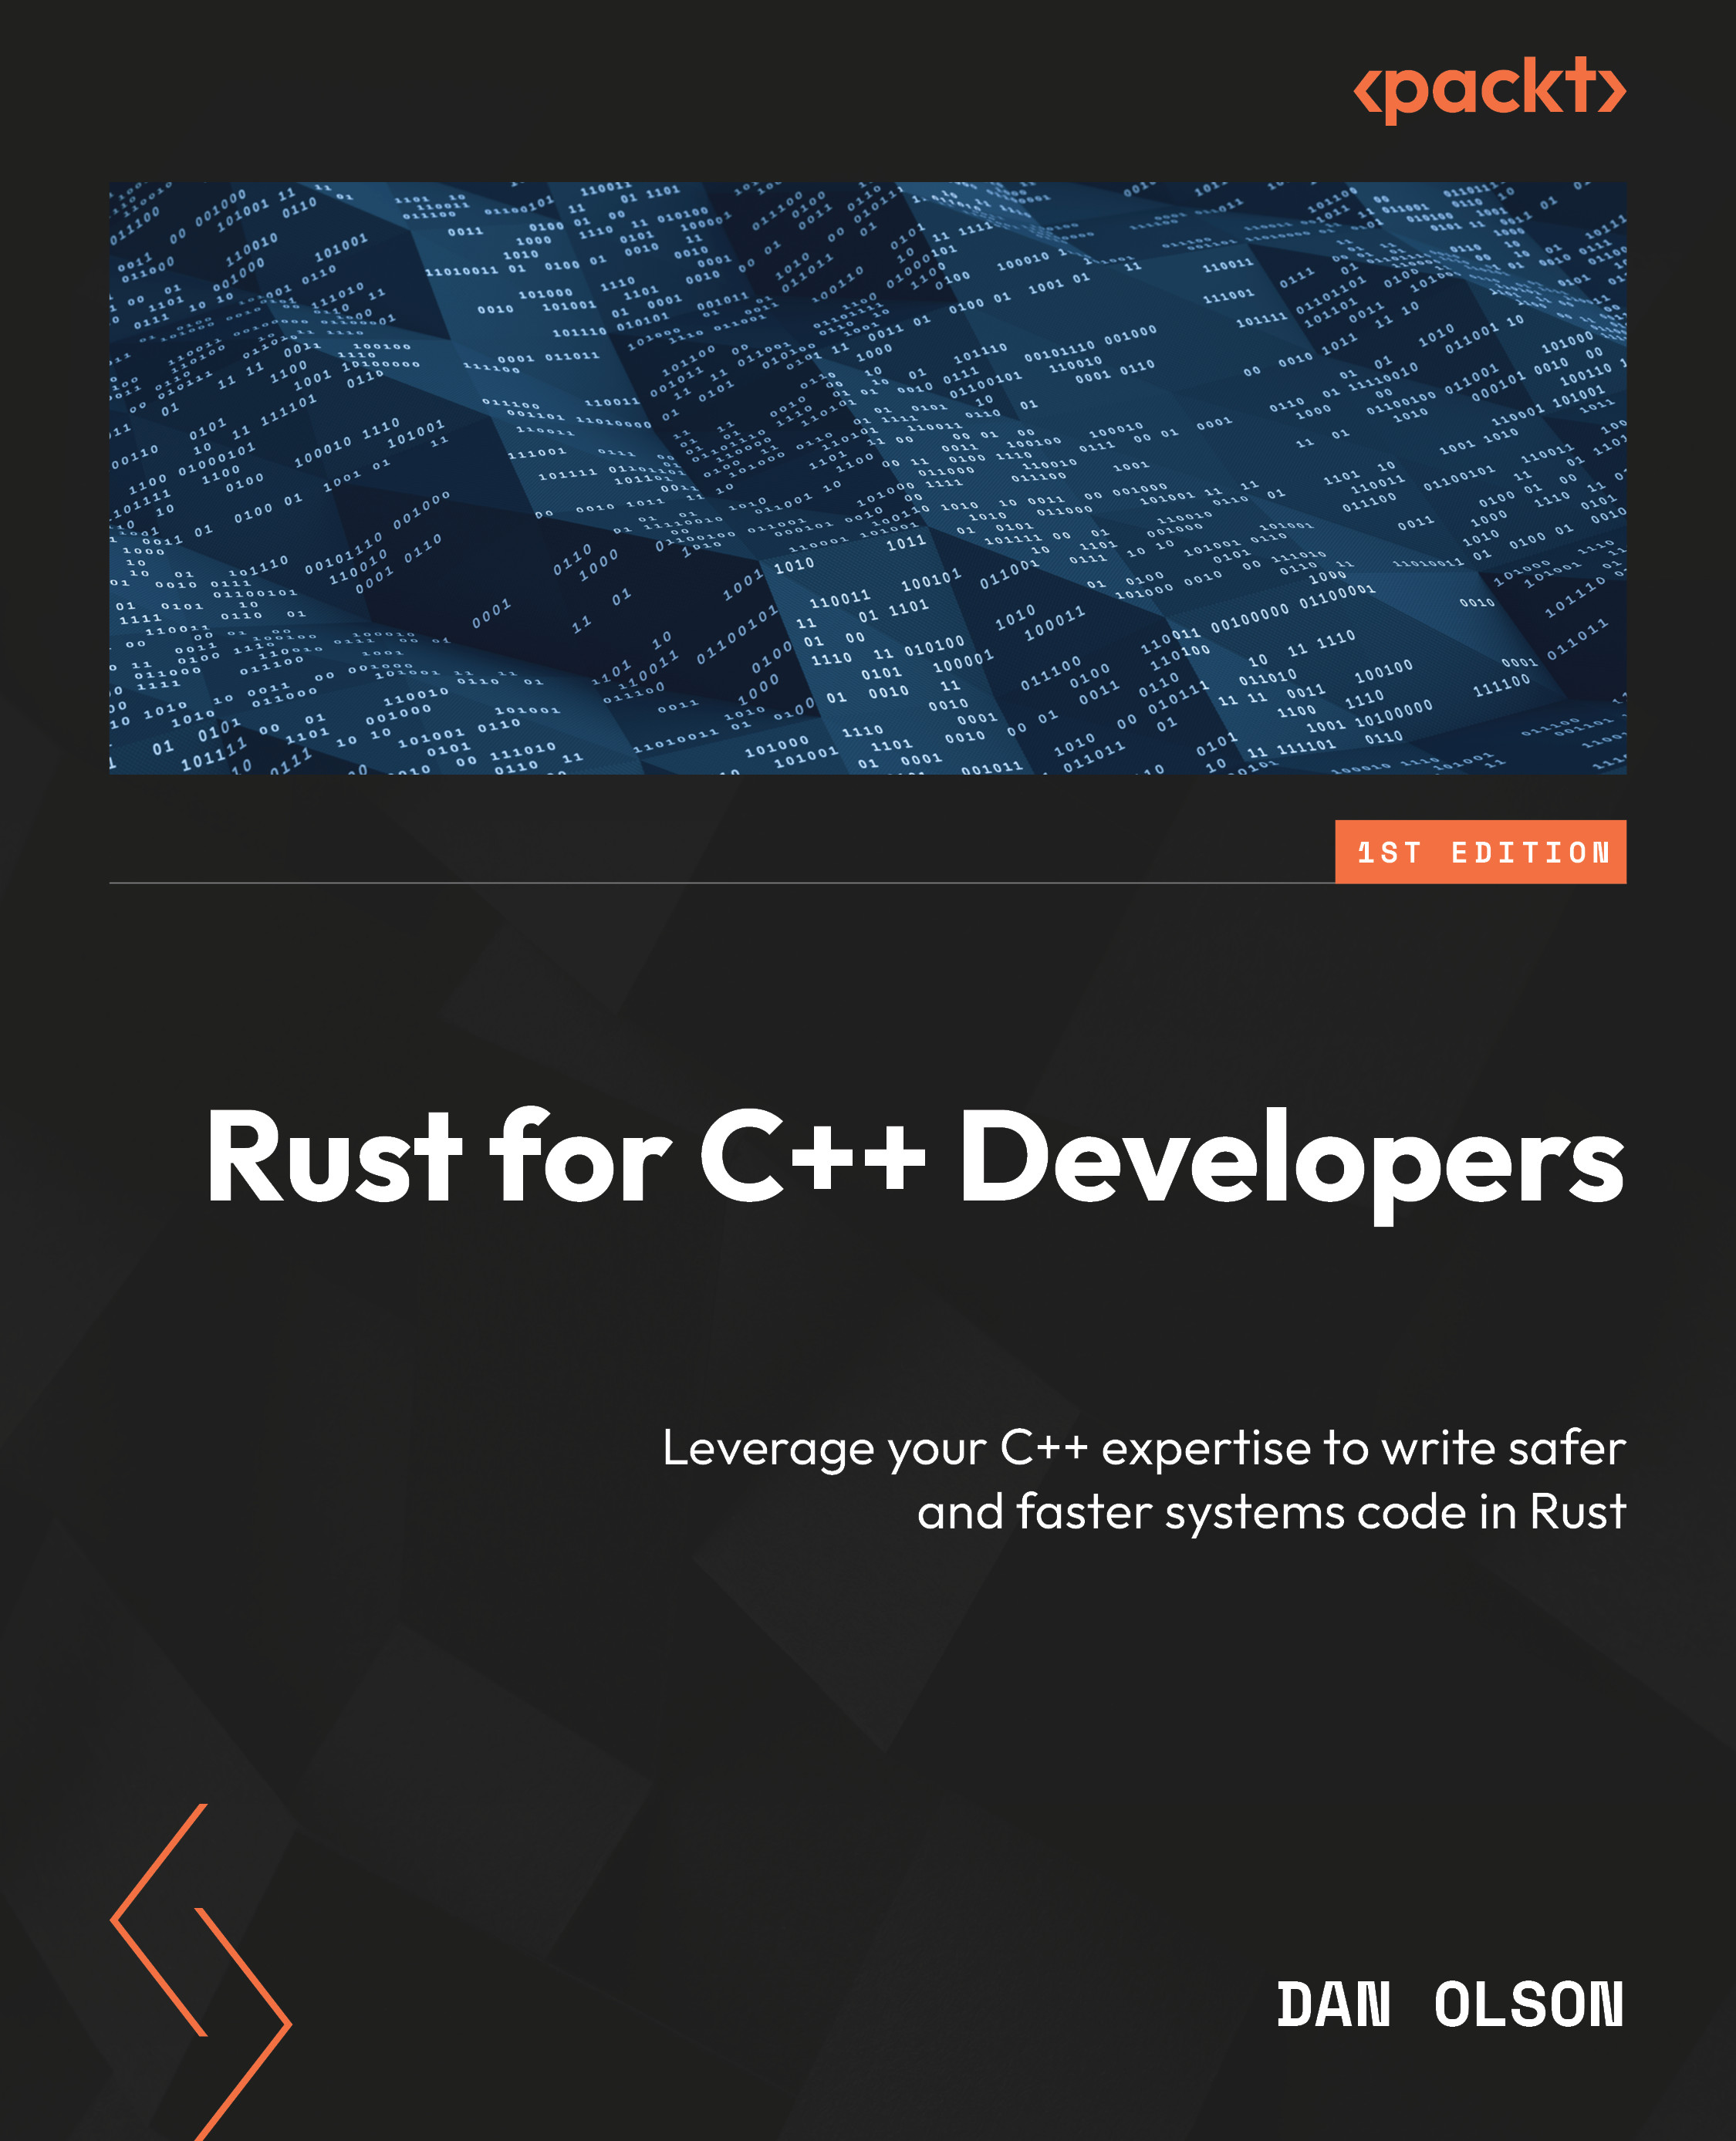
\includegraphics[width=\paperwidth,height=\paperheight,keepaspectratio]{images/cover.jpg}};
\end{tikzpicture}
\end{center}

\subfile{content/front/00-title}
\myFrontNoToc{content/front/01-copyright}
\subfile{content/front/11-dedication}

\newpage
\thispagestyle{empty}
\tableofcontents
\newpage

\myFront{贡献者}{content/front/03-contributors}

\myFront{前言}{content/front/04-preface}

\myPart{1}{理解 Rust 基础}{content/main/part1}

\myChapter{1}{为什么选择 Rust？}{content/main/01}

\myChapter{2}{使用 Rust 语法}{content/main/02}

\myChapter{3}{Rust 的安全模型}{content/main/03}

\myChapter{4}{用 Cargo 管理 Rust 项目}{content/main/04}

\myPart{2}{探索 Rust 标准库}{content/main/part2}

\myChapter{5}{数据结构}{content/main/05}

\myChapter{6}{读写文件}{content/main/06}

\myChapter{7}{理解迭代器}{content/main/07}

\myChapter{8}{面向对象编程}{content/main/08}

\myChapter{9}{在 Rust 中使用 C++}{content/main/09}

\myPart{3}{步入高级 Rust}{content/main/part3}

\myChapter{10}{Rust 中的优化}{content/main/10}

\myChapter{11}{Rust 中的多线程}{content/main/11}

\myChapter{12}{用宏进行元编程}{content/main/12}

\myChapter{13}{继续深入 Rust}{content/main/13}

\myAppendix{1}{搭建开发环境}{content/appendix/01}

\myChapter{15}{解锁你的专属权益}{content/main/15}

\myFront{你可能喜欢的其他图书}{content/back/01-other-books}

\myFront{索引}{content/front/index}
